%%%%%%%%%%%%%%%%%%%%%%%%%%%%%%%%%%%%

\section{点推定値と標本変動性}

%%%%%%%%%%%%%%%%%%%%%%%%%%%%%%%%%%%%

\subsection{点推定値と誤差}

%%%%%%%%%%%%%%%%%%%%%%%%%%%%%%%%%%%%

\begin{frame}
\frametitle{点推定値と誤差}

\begin{itemize}

\item 私たちはしばしば\hl{母集団のパラメータ}（母数）に関心を持つ。

\item 母集団全体からデータを収集することは難しいため、未知の母集団パラメータの推定に\hl{標本統計量}を\hl{点推定値}として使用する。

\item 推定の\hl{誤差} ＝ 母集団パラメータと標本統計量の差

\item \hl{偏り（バイアス）}とは、真の母集団パラメータを系統的に過大または過小に推定する傾向のことである。

\item \hl{標本誤差}とは、ある標本から次の標本へと推定値がどれだけ変動しやすいかを表す。

\item 統計学の多くは標本誤差の理解と定量化に焦点を当てており、\hl{標本サイズ}はこの誤差を定量化するのに役立つ。

\end{itemize}

\end{frame}

%%%%%%%%%%%%%%%%%%%%%%%%%%%%%%%%%%%

\begin{frame}
\frametitle{}

\dq{アメリカの各州からそれぞれ1,000人の成人を無作為に抽出したとする。各州の身長の標本平均は同じになると思うか、やや異なると思うか、それとも大きく異なると思うか？}

\soln{同じではないが、それほど大きな差はなく、やや異なる程度だろう。}

\end{frame}

%%%%%%%%%%%%%%%%%%%%%%%%%%%%%%%%%%%%

\subsection{点推定値の変動性を理解する}

%%%%%%%%%%%%%%%%%%%%%%%%%%%%%%%%%%%%

\begin{frame}
\frametitle{}

\begin{center}
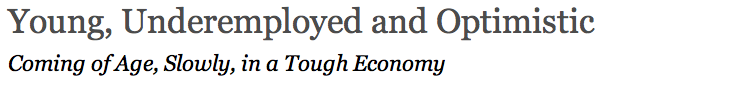
\includegraphics[width=0.95\textwidth]{5-1_point_est_sampling_var/figures/pew/pew1} \\
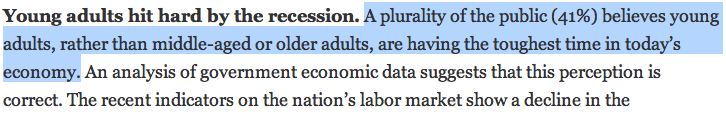
\includegraphics[width=0.95\textwidth]{5-1_point_est_sampling_var/figures/pew/pew2} \\
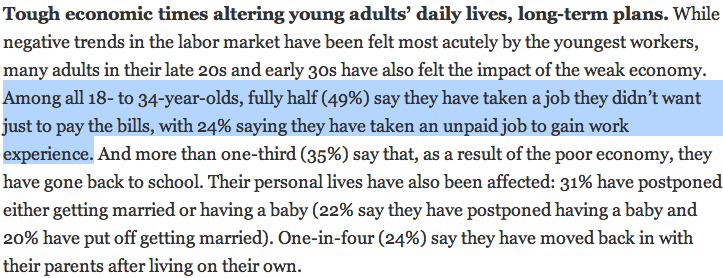
\includegraphics[width=0.95\textwidth]{5-1_point_est_sampling_var/figures/pew/pew3}
\end{center}

\ct{\webURL{http://pewresearch.org/pubs/2191/young-adults-workers-labor-market-pay-careers-advancement-recession}}

\end{frame}

%%%%%%%%%%%%%%%%%%%%%%%%%%%%%%%%%%%%

\begin{frame}
\frametitle{誤差の範囲（許容誤差）}

\begin{center}
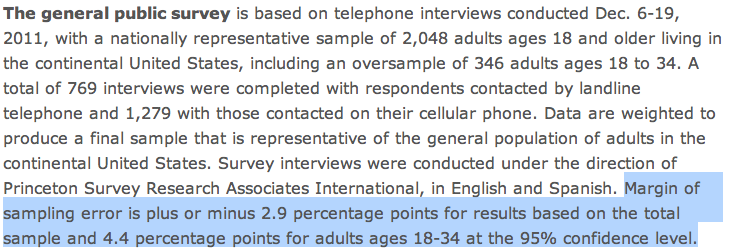
\includegraphics[width=0.95\textwidth]{5-1_point_est_sampling_var/figures/pew/pew4}
\end{center}

\begin{itemize}

\item 41\% $\pm$ 2.9\%：38.1\%から43.9\%の国民が、中年層や高齢者よりも若い成人が今日の経済で最も苦しんでいると考えていることを95\%の信頼度で確信している。

\item 49\% $\pm$ 4.4\%：18〜34歳の44.6\%から53.4\%が、請求書を支払うためだけに望まない仕事に就いたことがあると95\%の信頼度で確信している。

\end{itemize}

\end{frame}

%%%%%%%%%%%%%%%%%%%%%%%%%%%%%%%%%%%

\subsection{応用演習}

%%%%%%%%%%%%%%%%%%%%%%%%%%%%%%%%%%%

\begin{frame}
\frametitle{}

\dq{アメリカの成人で太陽光エネルギーの拡大を支持する割合が $p = 0.88$ であるとする（これが関心のあるパラメータである）。無作為に選ばれたアメリカの成人は、太陽光エネルギーの拡大を支持する可能性が高いか、低いか？}

\soln{より支持する可能性が高い。}

\end{frame}

%%%%%%%%%%%%%%%%%%%%%%%%%%%%%%%%

\begin{frame}
\frametitle{}

\dq{アメリカの成人全体の母集団にアクセスできない場合（これはよくある状況である）、太陽光エネルギーの拡大を支持するアメリカの成人の割合を推定するために、母集団から標本を抽出し、その標本割合を未知の母集団割合の最良の推定値として使用することが考えられる。}

\begin{itemize}

\item 母集団からアメリカの成人1,000人を復元抽出し、太陽光エネルギーの拡大を支持するかどうかを記録する。

\item 標本割合を求める。

\item クラスの各メンバーが得た標本割合の分布をプロットする。

\end{itemize}

\end{frame}

%%%%%%%%%%%%%%%%%%%%%%%%%%%%%%%%%%%

\begin{frame}[fragile]
\frametitle{}

\begin{beamerboxesrounded}[shadow = true, lower = code body]{}
{
\small
\begin{verbatim}

# 1. Create a set of 250 million entries, where 88% of
# them are "support" and 12% are "not".

pop_size <- 250000000
possible_entries <- c(rep("support", 0.88 * pop_size),
                      rep("not", 0.12 * pop_size))


# 2. Sample 1000 entries without replacement.

sampled_entries <- sample(possible_entries, size = 1000)

# 3. Compute p-hat: count the number that are "support",
# then divide by # the sample size.

sum(sampled sampled_entries == "support") / 1000

\end{verbatim}
}
\end{beamerboxesrounded}

\end{frame}

%%%%%%%%%%%%%%%%%%%%%%%%%%%%%%%%%%%

\begin{frame}
\frametitle{標本分布}

このプロセスを何度も繰り返して多くの $\hat{p}$ を得たとする。この分布を\hl{標本分布}と呼ぶ。

\begin{center}
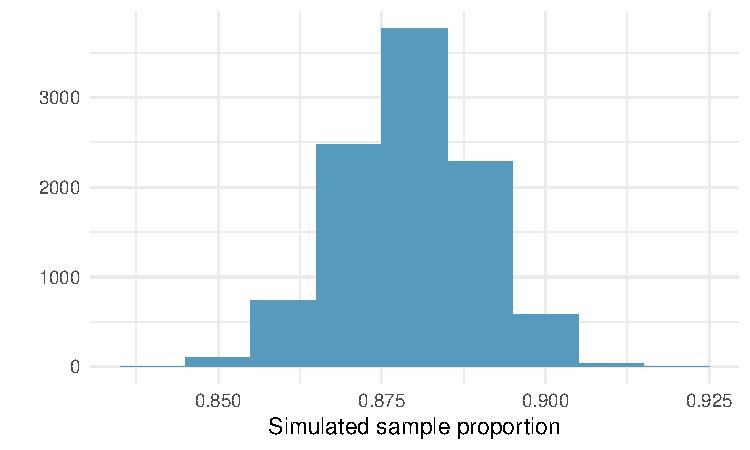
\includegraphics[width=0.6\textwidth]{5-1_point_est_sampling_var/figures/solar-power/solar-power-sampling.pdf}
\end{center}

\end{frame}

%%%%%%%%%%%%%%%%%%%%%%%%%%%%%%%%%%%

\begin{frame}
\frametitle{}

\dq{この分布の形と中心はどのようなものか？この分布に基づいて、真の母集団割合はどれくらいだと思うか？}

\begin{center}
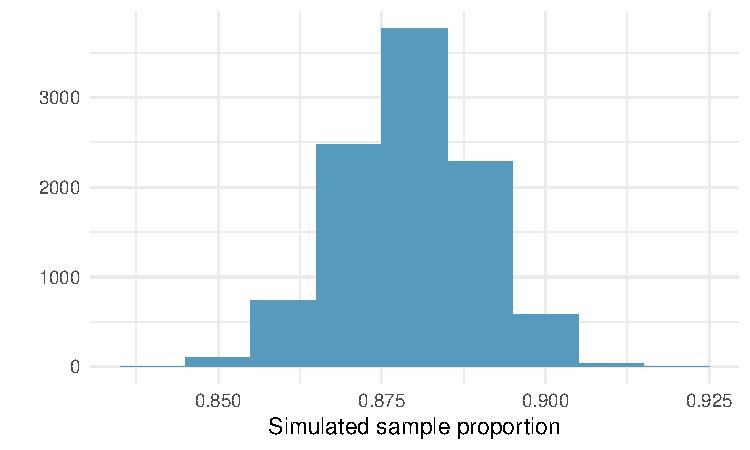
\includegraphics[width=0.6\textwidth]{5-1_point_est_sampling_var/figures/solar-power/solar-power-sampling.pdf}
\end{center}

$\:$ \\
\soln{この分布は単峰性でほぼ対称である。真の母集団割合の合理的な推測は、この分布の中心で、約0.88である。}

\end{frame}

%%%%%%%%%%%%%%%%%%%%%%%%%%%%%%%%

\begin{frame}
\frametitle{標本分布は実際には観察されない}

\begin{itemize}

\item 実際の応用では、標本分布を直接観察することは決してないが、点推定値はそのような仮想的な分布から得られるものとして常に考えることが有用である。

\item 標本分布を理解することで、実際に観察する点推定値の特性を明らかにし、理解することができる。

\end{itemize}

\end{frame}

%%%%%%%%%%%%%%%%%%%%%%%%%%%%%%%%

\subsection{中心極限定理}

%%%%%%%%%%%%%%%%%%%%%%%%%%%%%%%%%%

\begin{frame}
\frametitle{中心極限定理}

\formula{中心極限定理}
{標本割合は、母集団の割合 $p$ を平均とし、標準誤差を $\sqrt{\frac{p~(1-p)}{n}}$ とする正規分布にほぼ従う。
\[ \hat{p} \sim N \pr{ \text{平均} = p, SE = \sqrt{\frac{p~(1-p)}{n}} } \]
}

\begin{itemize}

\item 先ほど見た標本分布が対称で真の母集団割合を中心としていたことは偶然ではなかった。

\item $SE = \sqrt{\frac{p~(1-p)}{n}}$ の詳細な証明は省くが、$n$ が増加すると $SE$ が減少することに注目されたい。
\begin{itemize}
\item $n$ が増えるにつれて、標本はより一貫した $\hat{p}$ をもたらし、すなわち $\hat{p}$ 間の変動性が低くなる。
\end{itemize}

\end{itemize}

\end{frame}

%%%%%%%%%%%%%%%%%%%%%%%%%%%%%%%%%%%%

\begin{frame}
\frametitle{中心極限定理の適用条件}

中心極限定理を適用するためには、一定の条件が満たされなければならない：

\begin{enumerate}

\item \hlGr{独立性：}抽出された観測値は互いに独立でなければならない。\\

これを確認することは難しいが、以下の場合により可能性が高い：
\begin{itemize}
\item 無作為抽出・割り当てが行われている場合、および
\item 非復元抽出の場合、$n$ が母集団の10\%未満である場合。
\end{itemize}

\item \hlGr{標本サイズ：}観察された標本において、期待される成功数と失敗数がそれぞれ少なくとも10以上あること。

母集団割合が不明な場合（または仮定できない場合）、この条件を確認することは難しい。そのような場合は、観察された成功数と失敗数がそれぞれ少なくとも10以上あることを確認する。

\end{enumerate}

\end{frame}
%%%%%%%%%%%%%%%%%%%%%%%%%%%%%%%%%%

\subsection{中心極限定理の実際への応用}

%%%%%%%%%%%%%%%%%%%%%%%%%%%%%%%%%%

\begin{frame}
\frametitle{$p$ が未知の場合}

\begin{itemize}

\item 中心極限定理では $SE = \sqrt{\frac{p~(1-p)}{n}}$ とされており、$np$ と $n(1-p)$ がそれぞれ少なくとも10であることが条件だが、母集団割合 $p$ の値が不明なことが多い。

\item そのような場合は $p$ の代わりに $\hat{p}$ を代入する。

\end{itemize}

\end{frame}

%%%%%%%%%%%%%%%%%%%%%%%%%%%%%%%%%%%

\subsection{中心極限定理に関するさらなる詳細}

%%%%%%%%%%%%%%%%%%%%%%%%%%%%%%%%%%%%

\begin{frame}
\frametitle{$p$ が小さい場合}

\dq{真の母集団割合が $p = 0.05$ である母集団があり、この母集団からサイズ $n = 50$ の無作為標本を抽出するとする。各標本の標本割合を計算してこれらの割合をプロットした場合、この分布はほぼ正規分布になると予想されるか？なぜそうなるか、あるいはならないか？}

\soln{いいえ、成功・失敗条件が満たされていないため（$50 \times 0.05 = 2.5$）、標本分布がほぼ正規分布になるとは期待できない。
\begin{center}
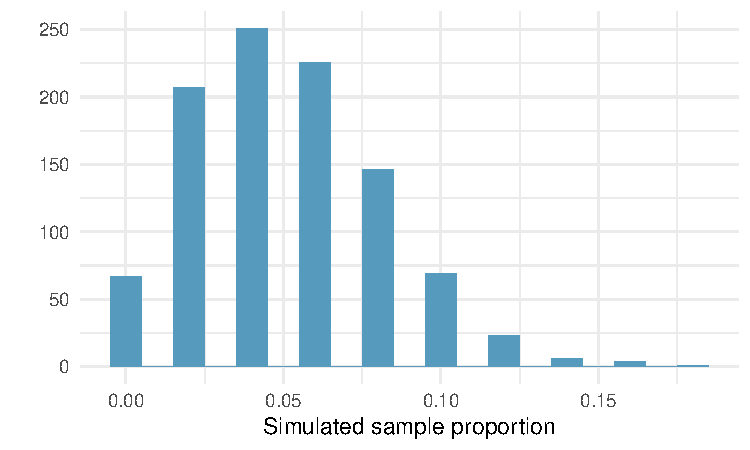
\includegraphics[width=0.55\textwidth]{5-1_point_est_sampling_var/figures/sf/low-p.pdf}
\end{center}
}

\end{frame}

%%%%%%%%%%%%%%%%%%%%%%%%%%%%%%%%%%%

\begin{frame}

\dq{$np$ および/または $n(1-p)$ が10未満の場合はどうなるか？}

\begin{center}
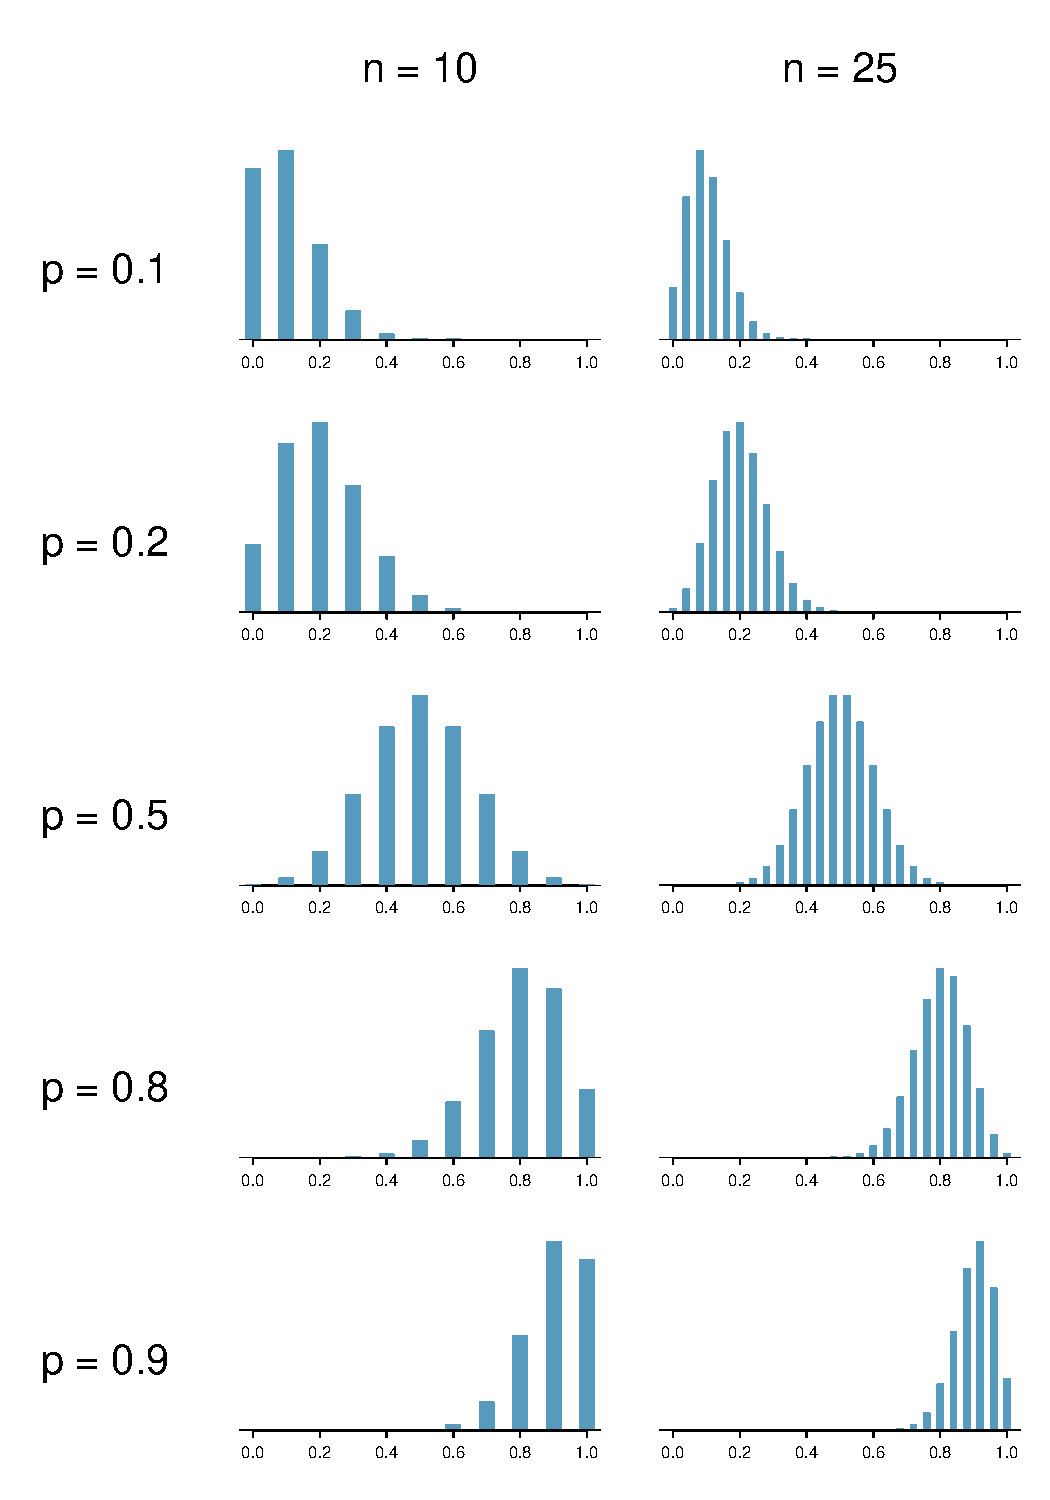
\includegraphics[width=0.45\textwidth]{5-1_point_est_sampling_var/figures/clt_prop_grid/clt_prop_grid_1.pdf}
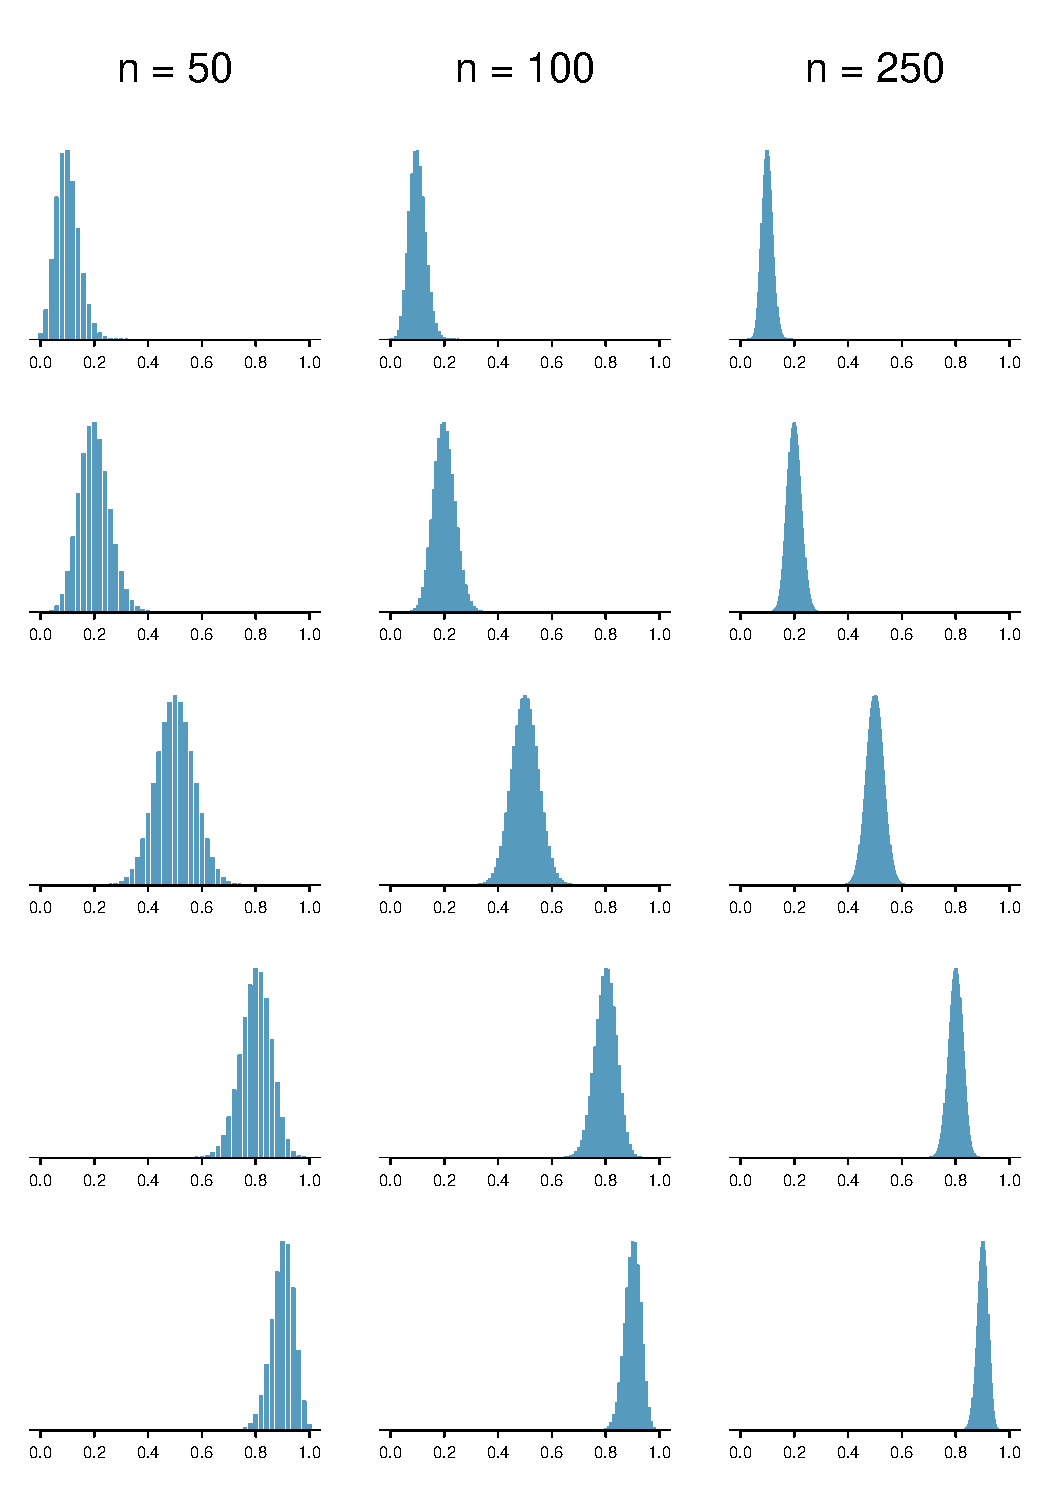
\includegraphics[width=0.45\textwidth]{5-1_point_est_sampling_var/figures/clt_prop_grid/clt_prop_grid_2.pdf}
\end{center}

\end{frame}

%%%%%%%%%%%%%%%%%%%%%%%%%%%%%%%%%%%

\begin{frame}
\frametitle{条件が満たされない場合…}

\begin{itemize}

\item $np$ または $n(1-p)$ のいずれかが小さい場合、分布はより離散的になる。
\item $np$ または $n(1-p)$ が10未満の場合、分布はよりゆがんだ形になる。
\item $np$ と $n(1-p)$ の両方が大きくなるほど、分布はより正規分布に近くなる。
\item $np$ と $n(1-p)$ の両方が非常に大きい場合、分布の離散性はほとんど見られなくなり、分布は正規分布にかなり近い形になる。

\end{itemize}

\end{frame}

%%%%%%%%%%%%%%%%%%%%%%%%%%%%%%%%%%%%

\subsection{他の統計量への枠組みの拡張}

%%%%%%%%%%%%%%%%%%%%%%%%%%%%%%%%%%%%

\begin{frame}
\frametitle{他の統計量への枠組みの拡張}

\begin{itemize}

\item 標本統計量を使ってパラメータを推定するという戦略は非常に一般的であり、割合以外の統計量にも適用できる戦略である。

\begin{itemize}
\item 大学の学生の無作為標本を抽出し、課外活動にいくつ参加しているかを聞いて、その大学の全学生が参加している課外活動の平均数を推定する。
\end{itemize}

\item この章の原則と一般的な考え方は、詳細が若干変わるとしても、他のパラメータにも適用される。

\end{itemize}

\end{frame}
